\solution 
Given that,
\begin{align}
    \vec{A} = \myvec{-3\\-5}
    \quad
    \vec{B} &= \myvec{3\\-5}
    \quad
    \vec{C} = \myvec{-4\\-3}
\end{align}
Given that $\vec{A},\vec{B},\vec{C}$ are collinear if
\begin{align}
    \text{rank}\myvec{
    1 & 1 & 1\\
    \vec{A} & \vec{B} & \vec{C} \\
    } &< 3 
    \label{eq:1.1.3,2}
\end{align} 
Let
\begin{align}
    \vec{R}&=\myvec{
    1 & 1 & 1
    \\
    -3 & 3 & -4
    \\
    -5 & -5 & -3
    } 
\end{align} 
The matrix $\vec{R}$ can be row reduced as follows,
\begin{align}
    \label{eq:matthrowoperations}
    \myvec{
    1 & 1 & 1
    \\
    -3 & 3 & -4
    \\
    -5 & -5 & -3
    }
     \xleftrightarrow[]{R_3 \leftarrow R_3+5R_1}
    \myvec{
    1 & 1 & 1
    \\
    -3 & 3 & -4
    \\
    0 & 0 & 2 
    }
    \\
     \xleftrightarrow[]{R_2\leftarrow R_2+3R_1}
    \myvec{
    1 & 1 & 1
    \\
    0 & 6 & -1
    \\
    0 & 0 & 2 
    }
\end{align}
There are no zero rows. So,
\begin{align}
    \text{rank}\myvec{
    1 & 1 & 1\\
    \vec{A} & \vec{B} & \vec{C} \\
    } &= 3 
\end{align}  
Hence, from \eqref{eq:1.1.3,2} the points $\vec{A},\vec{B},\vec{C}$ are not collinear. 

From Fig. \ref{fig1:Triangle}, We can see that $\vec{A},\vec{B},\vec{C}$ are not collinear .
\begin{figure}[h]
\centering
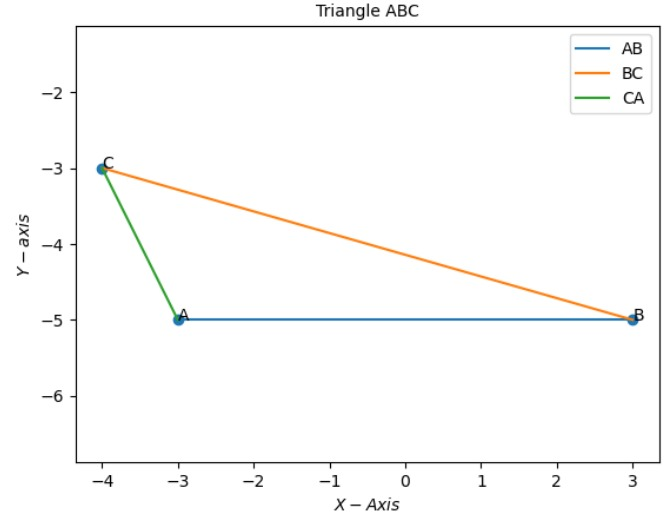
\includegraphics[width=\columnwidth]{figs/collinear.jpg}
\caption{$\vec{A},\vec{B},\vec{C}$ plot}
\label{fig1:Triangle}
\end{figure}

